\section{The challenges with \mup\ in practice} \label{sec:the_challenges_with_mup_in_practice}

% In this section we provide an analysis of the practical difficulties of using \mup. Despite its usefulness in various settings, \mup\ brings with it several challenges not evident in the exposition in Tensor Programs V\footnotemark. Some of these have been observed previously, while others are shown here for the first time.
% This analysis lays the groundwork for section \todocite, where we demonstrate solutions to these problems through \umup.

\footnotetext{As in other work, we use \mup\ as a shorthand for the method outlined in Tensor Programs V, including \mut. Strictly speaking, \mup\ ought only to refer to the parametrization outlined in Tensor Programs IV.}

\subsection{Not all training setups give \mut} \label{sec:challenges:mut}

Lingle \citep{Exploration_Of_Mu_Transfer} shows that directly applying \mup\ to a decoder LM fails to provide LR transfer across width. Given that the primary use of \mup\ in the literature has been LM training of this kind, this result suggests a significant limitation. How do we reconcile this with the strong LR transfer across width shown for language models in Tensor Programs V?

% The answer lies in the sensitivity of \mup\ to aspects of the training setup. Lingle further shows that \mut\ can be restored by removing all parameters from LayerNorms, and by changing AdamW \todocite to regular Adam \todocite. Similarly, the strong transfer shown in Tensor Programs V (Figure~4) can be attributed to aspects of its training setup.


\begin{figure}
    \centering
    \begin{subfigure}{\textwidth}
        \centering
        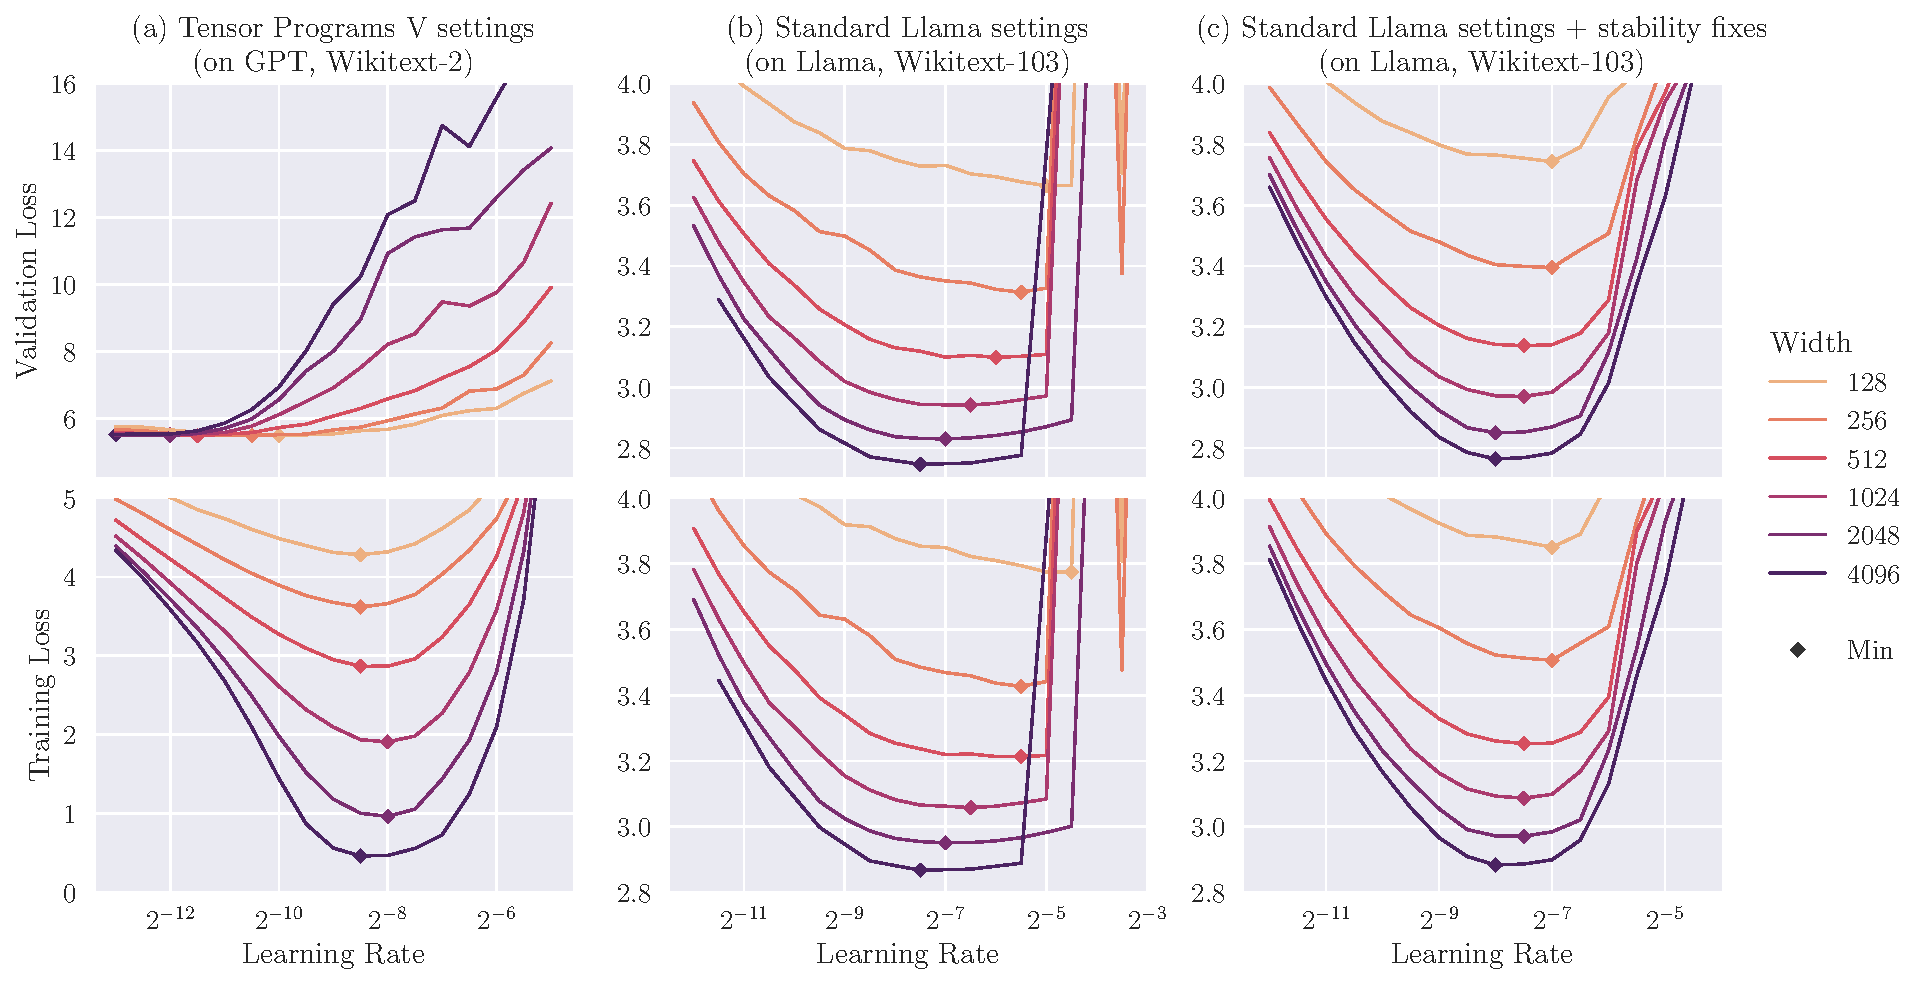
\includegraphics[width=\textwidth]{arXiv/figures/fig_TPV_improvements.pdf}
    % \vspace{1em}
    \end{subfigure}
    \caption{Effective \mut\ does not hold across all training setups.
    \textbf{(a)} We show strong transfer for the unrealistic setup used in Tensor Programs V (too many epochs; constant LR). \textbf{(b)} Moving to a more standard Llama training setup, transfer breaks down. \textbf{(c)} This is restored by the introduction of two stability fixes: non-parametric norms and independent weight decay.}
    % \caption{\textbf{(a)} LR transfer for decoder LMs (GPT) using the config from Tensor Programs V. This overfits due to the use of many epochs, which in turn changes transfer behavior and stops the use of validation loss. \textbf{(b)} The same experiment, but for a standard Llama training setup. The sharp increase in loss just after the optimum means small transfer errors can have catastrophic effects. \textbf{(c)} Introducing the non-parametric norms from \citep{Exploration_Of_Mu_Transfer} and independent weight decay from \citep{Small_Scale_Proxies} gives smoother degradation.}
    \label{fig:experiments:tpv_setup}
\end{figure}

We answer this \Cref{fig:experiments:tpv_setup}. The first training setup (a) is aligned with that used in Tensor Programs V (their Figure 4). There are several atypical aspects to their training setup, primarily the use of a constant LR schedule and a high number of epochs. This overfitting regime makes validation loss unusable, and transfer misleadingly good. When we remove these and shift to a standard Llama training setup (b), optimal HPs begin to drift with width. This confirms Lingle's findings that standard \mup\ is in fact a poor fit for modern LM training. We fix this (c) by the removal of parameters from LayerNorms/RMSNorms, as suggested by Lingle, and the introduction of \textit{independent} weight decay for AdamW, as suggested by Wortsman et al. \citep{Small_Scale_Proxies} \footnote{Lingle suggests independent weight decay is unstable, but we find it to be more so than Adam or standard AdamW.} (see \citep{AdamW_Weight_Decay} for further analysis). With these changes adopted, we recover the strong transfer shown in Tensor Programs V's experiments.

% In \Cref{fig:experiments:tpv_setup} we show the effect of these different training setups on transfer. We start with one similar to Tensor Programs V, though plotting validation as well as training loss. Validation loss is ultimately our target as this is what is used for \mut, but due to the many-epoch setup used by the authors, only the training loss can exhibit transfer. Focusing on training loss here may be justified if it can serve as a good proxy for validation loss, but we show in \Cref{fig:experiments:tpv_setup} that this is not the case: transfer behavior changes with overfitting, suggesting \mup\ should not be tested in the multi-epoch setting.
% We progress to standard Llama training on a large enough dataset to avoid overfitting. However this case also has a very undesirable property: sudden, severe increases in the loss at LRs beyond the optimum. This risks completely degrading training if transfer is slightly misaligned.
% These two changes give us more forgiving degradation with large LRs along with improved transfer---a further indication that care must be taken with one's training setup in order to make \mup\ work as expected.

\subsection{It's not clear which hyperparameters to sweep} \label{sec:challenges:which_hps}

The problem of selecting HPs to sweep can be framed as choosing a subset of the per-tensor $\alpha_W, \sigma_W, \eta_W$ HPs outlined in \Cref{sec:background:the_maximal_update_parameterization}, and grouping across/within layers. As shown in \Cref{table:mup_hps}, \mut\ experiments in the literature have done this in a variety ways. Practitioners have not justified these choices, appearing to rely on a mixture of precedent and intuition. We outline two major downsides to the lack of a principled approach.

Firstly, not all groupings of HPs are suitable. Consider the commonly-used global $\sigma_\mathrm{init}$ HP. At initialization the activations going into the FFN swish function have $\operatorname{std}(x_\mathrm{swish}) \propto \sigma_{W_\mathrm{gate}}$, whereas the self-attention softmax activations have $\operatorname{std}(x_\mathrm{attn}) \propto \sigma_{W_\mathrm{Q}}\sigma_{W_\mathrm{K}}$. A global $\sigma$ HP thus has a linear effect on the FFN and a quadratic effect on attention, suggesting that this grouping may be unideal.

Secondly, not all HPs are independent of one another. The key example of this is the interaction between $\sigma_W$ and $\eta_W$. The relative size of a weight update is determined by the ratio $\eta_W / \sigma_W$, not by either HP individually. Because of this, the optimal values for $\sigma$ and $\eta$ depend on each other, which we demonstrate empirically in \Cref{sec:experiments:hp_independence}. This can make the problem of HP search much harder, and may be why hundreds of random-search runs have been required for sweeps in the literature.

% Thirdly, the property of \mut\ is often demonstrated for a global $\eta$ HP, but has been studied much less for other HPs. As such, there is little evidence that most HPs have transfer under \mup\ in practice. Indeed in \todocite we show an important case where this fails to hold. Overall, our \umup\ scheme introduces a more principled approach to HP selection that addresses the above issues.

\subsection{Base shape complicates usage}

Most practitioners are unlikely to require alignment with an SP model, in which case it is unclear what $\basewidth$ (and $\basedepth$) should be used. The literature has aligned on a standard $\basewidth$ of $256$ (see \Cref{table:mup_hps}), but this appears to lacking a principled motivation---though the fact that they are not dropped entirely suggests they may be beneficial under \umup.

Implementing base-shape HPs (see \Cref{eq:abc_mup_absolute}) can also add complications from an engineering perspective. The proposed implementation in the $\texttt{mup}$ library \citep{Mup_Library} reflects this, requiring an extra `base' model to be created and the original model to be re-initialized. This can interact awkwardly with other model-transforms for features like quantization, compilation, etc:

\vspace{0.3em}
\codefig{base_shapes.py}

% A base model is created alongside the target model, which is then used to re-scale it. This extra initialization and re-initialization breaks from the standard approach to model creation in PyTorch, and as a result may interact awkwardly with other model-wrappers for features like distributed training, quantization and compilation.

\subsection{\mup\ appears to struggle with low-precision}

Finally, we note an interesting contradiction observed in the relationship between \mup\ and low-precision. One of the stated aims for \mup\ is that its activations have $\Theta(1)$-sized coordinates in the limit \citep[Desiderata J.1]{Tensor_Programs_V}. This desideratum is specifically given in order that values can be represented using finite-range floating-point numbers \citep[Section 3]{Tensor_Programs_IV}.
Yet despite numerical stability being central to the theory underlying \mup, this is not leveraged to ensure that \mup\ models can \textit{actually} be trained in low-precision. Indeed, for the LLM runs in Tensor Programs V the SP model trains successfully in FP16, while the \mup\ model diverges (attributed to underflow of gradients). We remedy this with \umup.